%%%%%%%%%%%%%%%%%%%%%%%%%%%%%%%%%%%%%%%%%%%
% WARNING: Two pdflatex runs should be done each time, to update correctly LastPage    %
%%%%%%%%%%%%%%%%%%%%%%%%%%%%%%%%%%%%%%%%%%%

\documentclass[12pt, a4, hidelinks]{article}

\usepackage{ucs}
\usepackage[utf8x]{inputenc}
\usepackage[english]{babel}

\usepackage{siunitx}

\usepackage{graphicx}
\graphicspath{ {./images/} }

\usepackage{geometry}

\usepackage{fancyhdr}
\usepackage{lastpage}

\pagestyle{fancy}
\fancyhf{}
\renewcommand{\headrulewidth}{0pt}
\cfoot{Page \thepage \hspace{1pt} of \pageref{LastPage}}

\usepackage{hyperref}                           
\usepackage{xcolor}                             
%\usepackage{algorithm}
%\usepackage{algpseudocode}

\usepackage[linesnumbered,ruled,vlined]{algorithm2e}
%\usepackage{algorithmic}
\SetKwComment{Comment}{/* }{ */}
\hypersetup{                                     
	%colorlinks,                                    
	%linkcolor={red!50!black},                 
	citecolor={blue!50!black},                  
	urlcolor={blue!80!black}
}                                                
\usepackage{xurl}  

\begin{document}

\newgeometry{left=1in,right=1in,top=1in,bottom=1in}
\noindent \rule{\textwidth}{3pt}
\begin{center}
	{\bf \Large{Final Report - Sudoku on AVR}}\\
	ACE411-Embedded Microprocessor Systems \\
	Winter semester of academic year 2021-2022
	\rule{\textwidth}{0.2mm} 
	\begin{tabular}{l r}
		Kallinteris Andreas:& 2017030066 \\ 
		Lioudakis Emmanouil:      &2018030020 
	\end{tabular} \vrule \hspace{3mm}
	\indent	Team number on eclass:  5
	\rule{\textwidth}{1pt}
\end{center}

\section*{Introduction}
The project's purpose is to implement a program to solve a $9\times9$ sudoku grid on STK500. The interface used is a serial port (RS232), through which the development board receives commands and data (in ASCII format) and transmits data and messages. The 8 LEDs available on the board are also used, to display the progress of the solving procedure. An optimized algorithm for solving has been developed, to achieve fast solving time.


\section*{Description of the program}

\subsubsection*{The sudoku solving algorithm}
The sudoku solver baseline for the fist 8 rows is a general purpose DFS algorithm (with pruning invalid cases), where profiling indicated that the biggest time cost is the routine for pruning (finding which are the valid values for a cell).
And in order to minimize that cost, the calculations for pruning a cell are computed once and cached.

\noindent Lastly, after the first 8 rows are solved the last row is trivially solved.

\begin{algorithm}[H]
\SetKwInput{KwInput}{Input}                % Set the Input
\DontPrintSemicolon
	\KwInput{$lenght \gets 9$, $empty\_cell \gets 0$}
	\KwData{board[$lenght$][$lenght$]}

% Set Function Names
	\SetKwFunction{Ffirst}{solve\_first\_8\_rows}
	\SetKwFunction{Flast}{solve\_last\_row}
	\SetKwFunction{Fsolve}{solve}

	\SetKwProg{Fn}{Function}{:}{}
	\Fn{\Ffirst{$start\_index = 0$}}{
		\For{$i \gets start\_index$ \KwTo $lenght \times (lenght-1)$}{
			$y_{cord} \gets i / lenght$ \Comment*[r]{Computed using a LUT}
			$x_{cord} \gets i \% lenght$\Comment*[r]{Computed using a LUT}
			\If{$board[y_{cord}][x_{cord}] = empty\_cell$}{
				\Comment*[r]{list\_of\_possible\_values is trivial function going over the row, collumn and block of the existing cell}
				\For{$k \gets list\_of\_possible\_values(i)$}{
					$board[y_{cord}][x_{cord}] \gets k$\;
					\If{solve\_first\_8\_rows(i+1)}{
						\KwRet true;
					}
					$board[y_{cord}][x_{cord}] \gets empty\_cell$\;
				}
				\KwRet false;
			}
		}
		\KwRet true \Comment*[r]{reaching here means it has solved the first 8 rows}
	}\;

	\SetKwProg{Fn}{Function}{:}{}
	\Fn{\Flast{}}{
		$y_{cord} \gets lenght-1$\;
		\For{$x_{cord} \gets0$ \KwTo $lenght-1$}{
			$board[y_{cord}][x_{cord}] \gets last\_row\_remaing\_value(x_{cord})$\;
		}
	}\;

	\SetKwProg{Fn}{Function}{:}{}
	\Fn{\Fsolve{}}{
		solve\_first\_8\_rows()\;
		solve\_last\_row()\;
	}
\end{algorithm}

\subsubsection*{Controlling the LED progress bar}
To update the LEDs that show the progress of solving, there were two options. The first one was updating the PORTA register every time we change the value of a cell and the second one was refreshing the LEDs with a 30Hz frequency. The former option would consume many clock cycles (because on every PORTA update, its new value is read from flash, which needs 3 clock cycles many times each second), when the latter would consume those 3 cycles only 30 times per second. The latter was preferred, using Timer/Counter1.

\subsubsection*{USART interfacing}
As the assignment states, the serial port is configured at 9600 baud, 8 data bits, 1 stop bit and no parity.
\subsubsection*{Receiving from the serial port}
When a character is sent to the serial port, the USART\_RXC interrupt is triggered. In the interrupt handler, based on the receiver character, if it is a command character, a flag is set, else if it is a number it is stored in the memory. After receiving the line-feed character, the command is executed. \\
It is important to note that in the case of ``play'' command, the interrupt service routine does not call the solving function, but simply sets the solving flag and returns. This is done to return back as fast as possible, and then start solving with the interrupts enabled (when the ISR is called, the interrupts are disabled until it returns). In that way, while solving a break or a debug command can be received and executed (by interrupting the solving function). If the ISR called the solve function, until completing solving, the interrupts would be disabled, and any new characters from the serial port would not be read.

\subsubsection*{Transmitting to the serial port}
To transmit a character, a polling procedure is used. A loop is done to wait until the UDR register gets empty and then is written the characted to be transmitted. In fact, in this project, polling is not affecting the system's efficiency, because the baud rate is extremely low, so the UDR register will be empty, every time we want to transmit a character (every 10000 clock cycles approximately). So, for example the ``OK'' sending is done inside the USART interrupt handler in the case of an ``AT'' command. This is not a problem, because the communication protocol described in the assignment states that the computer will wait for the reply before sending a new command.

\section*{Microchip Studio configuration - Compilation process}
Since the code is written using the C++ language (using newer standards than the supported from Microchip Studio by default), some modifications should be done to the default settings of a new C++ project.  \\
Firstly, add the symbol ``AVR'' to the compiler’s defined symbols:\\
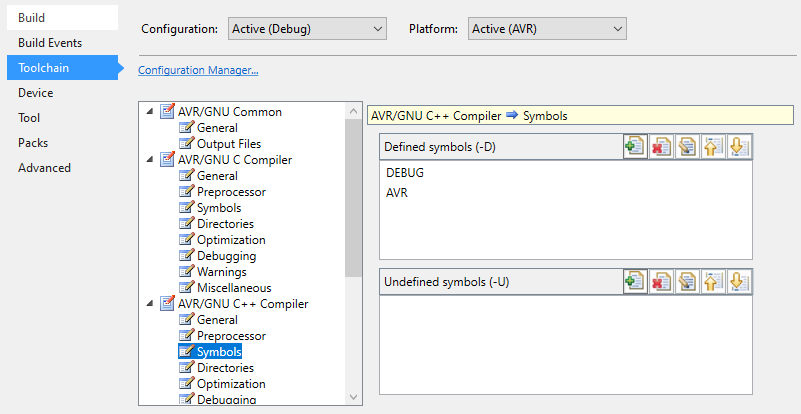
\includegraphics[scale=0.75]{CPP_AVR_SYMBOL.png} \\
Secondly, add the flag ``-std=c++17'' to the compiler’s flags:\\
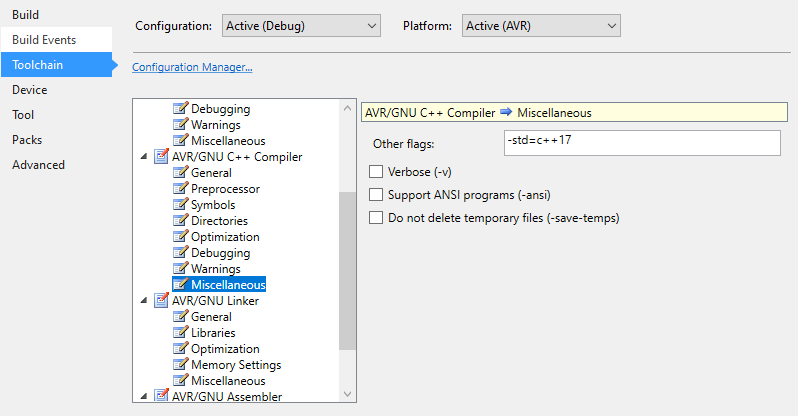
\includegraphics[scale=0.75]{CPP_STD_17.png}  \\
The optimization level should be set to ``-O2 (Optimize more)''.\\
Finally, the SIMULATION\_MODE should be defined (by uncommenting the line 25 of sudoku.h). When it is defined, the program will read from TCNT2 instead of UDR and will redirect its output from UDR to TCNT0. By doing that, the program can be simulated with the provided stimuli files. \\
The makefile should not be used with Microchip Studio, but only when using gnu-toolchain on linux system.

\section*{Resource usage}
After compiling the code, the following resource usage is reported: \\
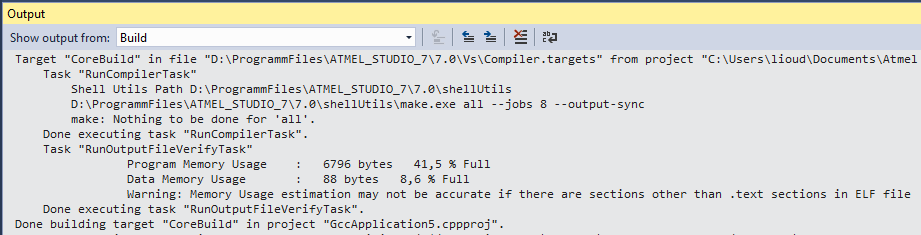
\includegraphics[width = \textwidth]{RESOURCES.png} 

\subsubsection*{Program memory (flash)}
Except from the code, two arrays (look up tables) are stored in flash: 
\begin{itemize}
\item The led\_bar\_LUT (defined in sudoku.h), which contains the decoding data for the LED progress bar (holds 82 bytes).
\item The div\_9\_LUT (defined in LUT.hpp), which contains pre-calculated value to make the solving proccess faster (holds 162 bytes).
\end{itemize}
The rest bytes (6888-82-162 = 6644) are reserved by the code instructions.

\subsubsection*{Static RAM (SRAM)}
The global variables used to control the serial port are the struct of flags for the received character(12 bits or 2 bytes), the union for the X counters (1 byte), the union for the Y counters (1 byte) and the counter for the arguments (1 byte). The rest of the 88 bytes are used for the base\_board object (an instance of the sudoku class). Inside this object is stored the 9x9 sudoku grid as a two dimensioned array of unsigned integers. \\
During the solving process, the solver uses up to 790 bytes, leaving 146 bytes for context switching during interrupts.

\section*{Simulation in Microchip Studio, using stimuli files}
Three stimuli files are submitted with the code (in the folder STIMULI\_FILES):
\begin{itemize}
\item simple\_solve.stim, which feeds the program with one sudoku board (the one shown in the assignment), waits until the sudoku is solved and sends the results back.
\item break\_debug\_test.stim, which feeds the program with the same sudoku board as above, but while solving, a ``break'' command stops the solving process, and using the ``debug'' command, the contents of some cells are read.
\item two\_sudokus.stim, which feeds the program with two sudoku boards, one after another. After solving the first and sending back the results, a ``clear'' command is executed and then the grid is filled with the second sudoku, it is solved and the results are sent back to the serial port.
\end{itemize}
Using the Microchip Studio debugging tools (Run To Cursor and Step Into) and by watching the memory contents (e.g. the values that are completed each moment in the sudoju grid, or if the flag bits are set to true/false), the functionality of the program can be evaluated.

\section*{Testing the code on real hardware (STK500)}
\subsubsection*{Using PuTTY}
Three tests have been done on hardware using PuTTY. The content of the PuTTY terminal is provided in the following files (in the folder PUTTY\_LOGS):
\begin{itemize}
\item simple\_solve\_tty.log, which feeds the program with one sudoku board (the one shown in the assignment), waits until the sudoku is solved and sends the results back.
\item break\_debug\_tty.log, which feeds the program with a difficult sudoku board (generated with the interface program, to slow the solving process and have the time to give manually a break command), but while solving, a ``break'' command stops the solving process, and using the ``debug'' command, the contents of some cells are read.
\item two\_sudokus\_tty.log, which feeds the program with two sudoku boards, one after another. After solving the first and sending back the results, a ``clear'' command is executed and then the grid is filled with the second sudoku, it is solved and the results are sent back to the serial port.
\end{itemize}
On each file, an identifier is placed in the start of each line, to show who sent this command ([PC] or [STK]).\\
Important note: While configuring the serial connection in PuTTY, the flow control can be set either to ``None'', or to ``XON/XOFF'' without any problem. Even when using XON/XOFF, the baud rate is so low, so the buffers of the two communicating devices (the PC and the STK) will never overflow.

\subsubsection*{Performance analysis}
To obtain an image of the algorithm's efficiency, the interface program was used. One hundred random boards of each difficulty level were generated and solved, using a batch file (perf\_analysis.bat). With a simple C program (file\_parser.c), the mean value and the standard deviation of solving time is calculated:
\begin{center}
\begin{tabular}{ |l|c|c|c|c| } 
 \hline
                                      & Easy         & Medium & Hard & Ultra  \\  \hline
Mean value (msec)           &  0.461918  &  \ 4.439484   &  18.620610       &  15006.633687        \\ \hline
Standard deviation (msec) &  1.063388  & 14.304317   & 36.208134        &  37863.171875         \\ \hline
\end{tabular}
\end{center}
\noindent The tests were done on 19 December 2021, using the version 1.5 of the interface. Although some boards are generated in a way to defeat backtracking (and therefore need more time to be solved), the results give an approximation of the needed time.

\noindent The GitHub repository \url{https://github.com/elioudakis/HRY411_Performance_Analysis} contains the batch file, the file parsing program and the log files produced. The log files are not submitted on eclass, because of their size (8 MB).

\section*{STK500 configuration}
The STK500 development board we have received has installed the ATmega16L microcontroller, which is fully compatible with the ATmega16 used in Microchip Studio. PORTA is fully functional, and therefore connected to the LEDs. An external crystal of 10MHz is used. Since ISP (In System Programmer) programming mode is used, the following jumpers are mounted:
\begin{description}
\item[VTARGET] mounted, to use the on-boars supply voltage.
\item[AREF] mounted, to use the AVR's AREF as reference volatge for the A/D converter on AVR. Although the A/D converter is not used in this project, the jumper is mounted, because this is the default setting.
\item[RESET] mounted, to be able to use the on-board reset button.
\item[XTAL1] mounted, to use the external crystal.
\item[OSCSEL] mounted to pins 2 and 3 to use the on-board crystal signal as clock signal.
\end{description}
The fuses configuration of the microcontroller is described in the file ``fuses\_config.conf''.

\section*{Conclusion}
The present project is a great example of designing an embedded system with real-time requirements. A simple sudoku solving algorithm designed for general purpose microprocessors (which have clock frequency of GHz), would not be efficient on a microcontroller (which has a clock frequency of several MHz). So it had to be optimized, and some values have been precalculated, to achieve a fast solving time. Additionally, two real-time requirements had to be implemented, the communication via the RS232 port and the LED interfacing, using the microcontroller's interrupts and internal modules (timers).

\end{document}
